\documentclass[12pt]{extarticle}
\usepackage[letterpaper, left=0.75in, right=0.75in, top=0.75in, bottom=0.6in,
  headheight=16pt, headsep=10pt, footskip=24pt]{geometry}
\usepackage{fontspec}
\setmainfont{texgyreheros}[Extension=.otf, UprightFont=*-regular,
  BoldFont=*-bold, ItalicFont=*-italic, BoldItalicFont=*-bolditalic]
\usepackage{tikz}
\usetikzlibrary{shapes.geometric}
\usepackage{fancyhdr}
\pagestyle{fancy}
\fancyhf{}
\fancyhead[L]{Week 8 / Rook race and Nim / Game boards}
\fancyfoot[L]{Bellingham Math Circle / Week 8 / F08-MAT-v1}
\fancyfoot[R]{\thepage}
\renewcommand{\headrulewidth}{0pt}
\setlength{\parindent}{0pt}
\setlength{\parskip}{0pt}
\hyphenpenalty=10000
\exhyphenpenalty=10000
\begin{document}
\raggedright
\textbf{8-by-8 game board: print 7 copies (2 for each table, 1 spare).}

\vspace{0.05in}
{\small Print single-sided at 100\% (\emph{Actual size}, not \emph{Fit to page}). Check one sheet with a ruler before printing the rest: the line under the board must measure 10 cm and each square 1 inch.\par}

\vspace{0.14in}
\noindent\makebox[\textwidth][c]{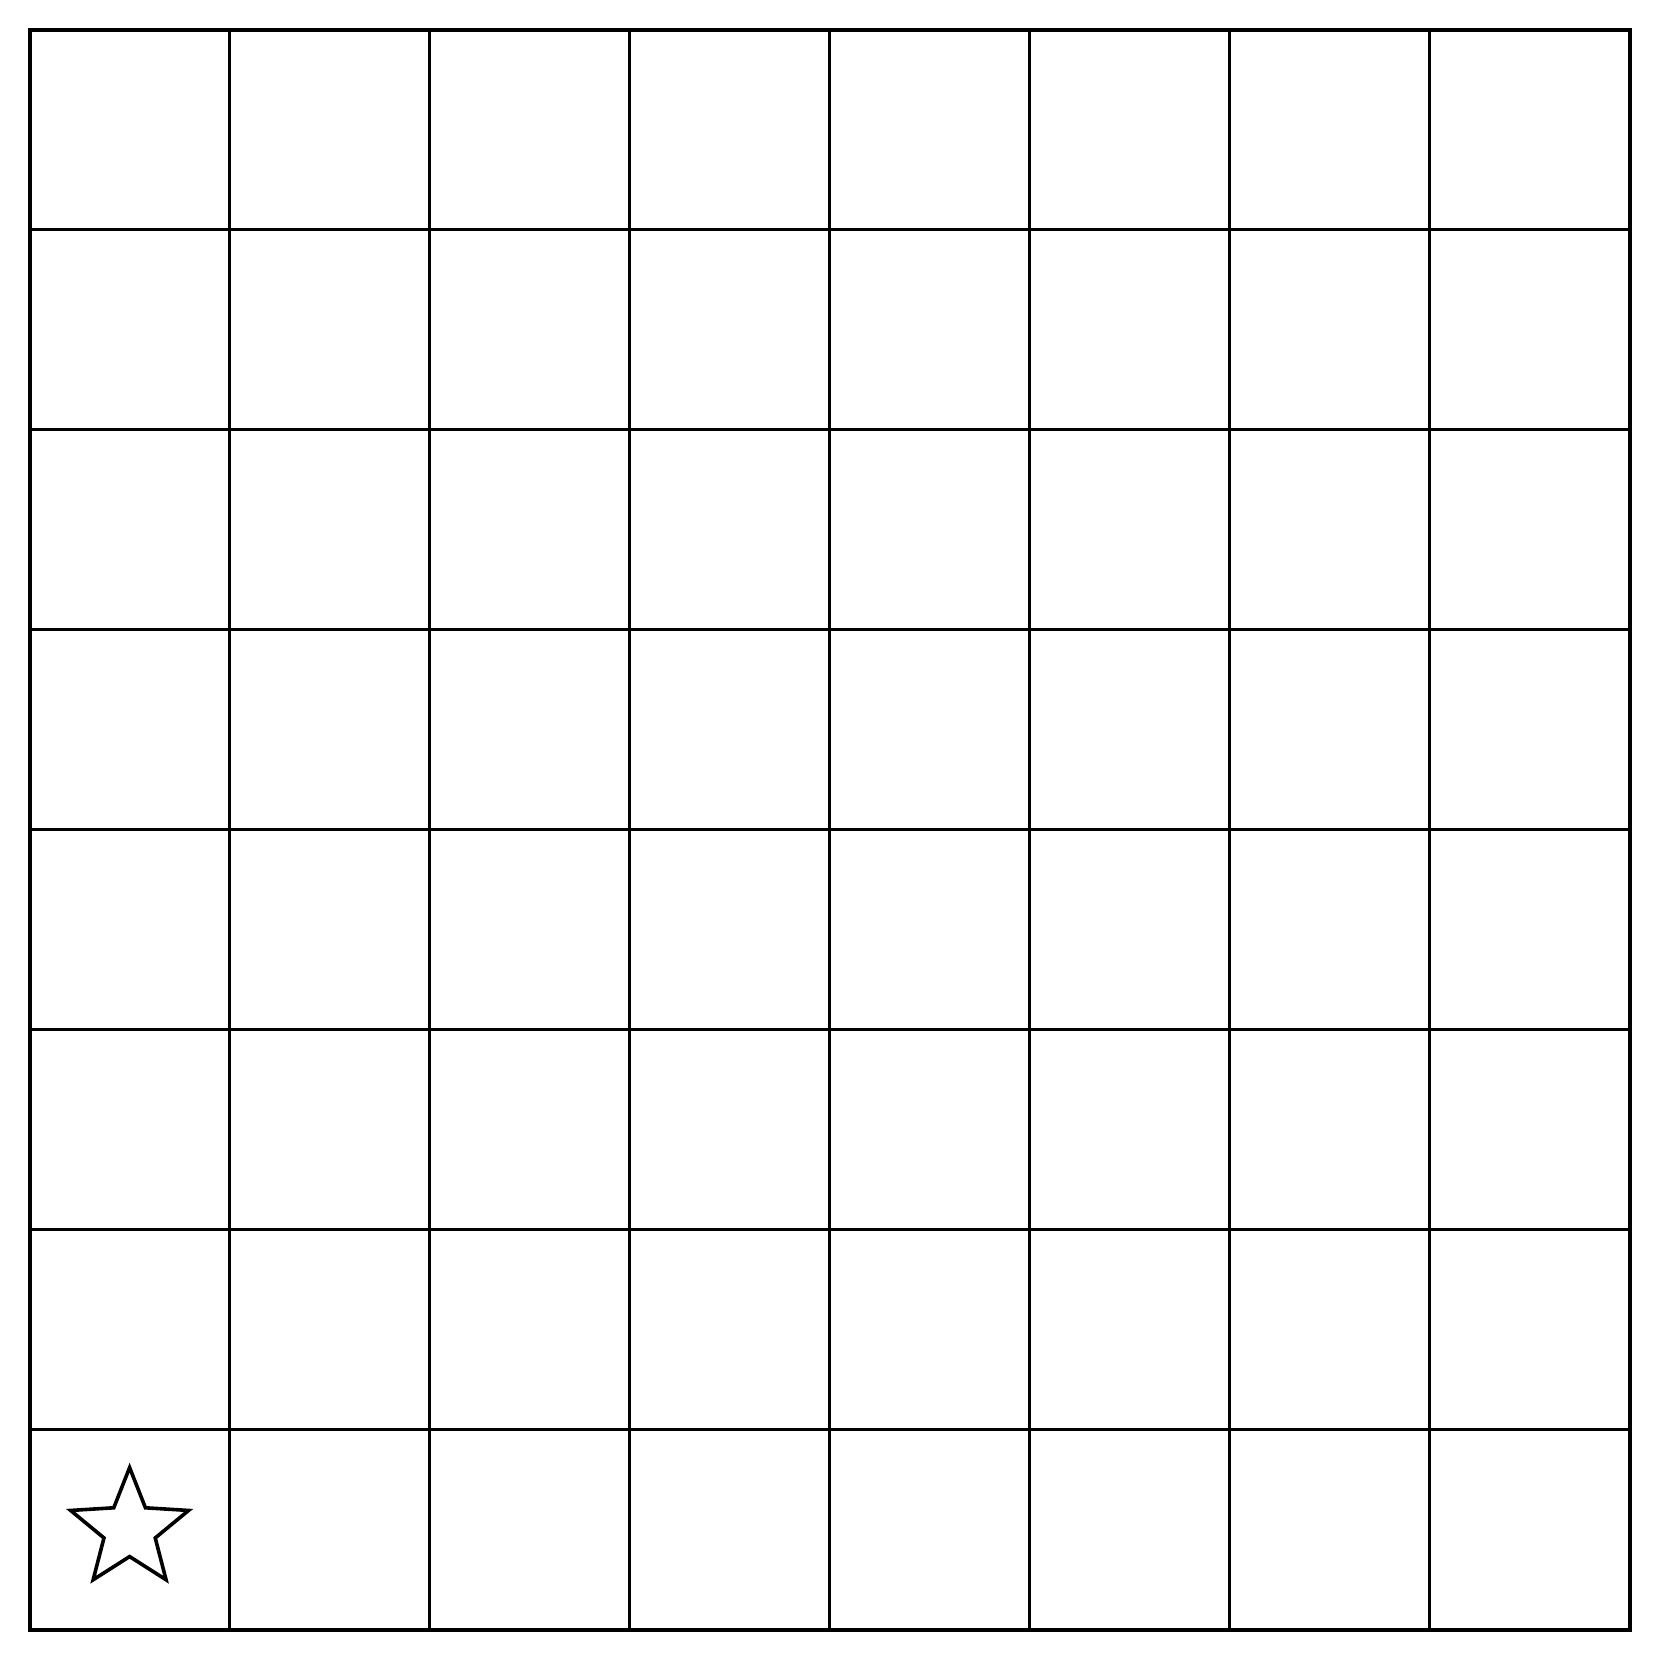
\begin{tikzpicture}[x=1in,y=1in]
\draw[line width=0.9pt] (0,0) grid[step=1] (8,8);
\draw[line width=1.4pt] (0,0) rectangle (8,8);
\node[star, star points=5, star point ratio=2.3, draw=black, line width=1.3pt, inner sep=0pt, outer sep=0pt, minimum size=0.620in] at (0.5,0.5) {};
\end{tikzpicture}}

\vspace{0.2in}
\noindent\makebox[\textwidth][c]{
\begin{tikzpicture}[x=1cm,y=1cm]
\draw[line width=1pt] (0,0) -- (10,0);
\draw[line width=1pt] (0,-0.2) -- (0,0.2);
\draw[line width=1pt] (10,-0.2) -- (10,0.2);
\node[anchor=west] at (10.3,0) {10 cm};
\end{tikzpicture}}

\newpage
\textbf{5-by-5 game board: print 3 copies (2 for the grades 2--3 table, 1 spare).}

\vspace{0.05in}
{\small Print single-sided at 100\% (\emph{Actual size}, not \emph{Fit to page}). Check one sheet with a ruler before printing the rest: the line under the board must measure 10 cm and each square 1 inch.\par}

\vspace{0.14in}
\noindent\makebox[\textwidth][c]{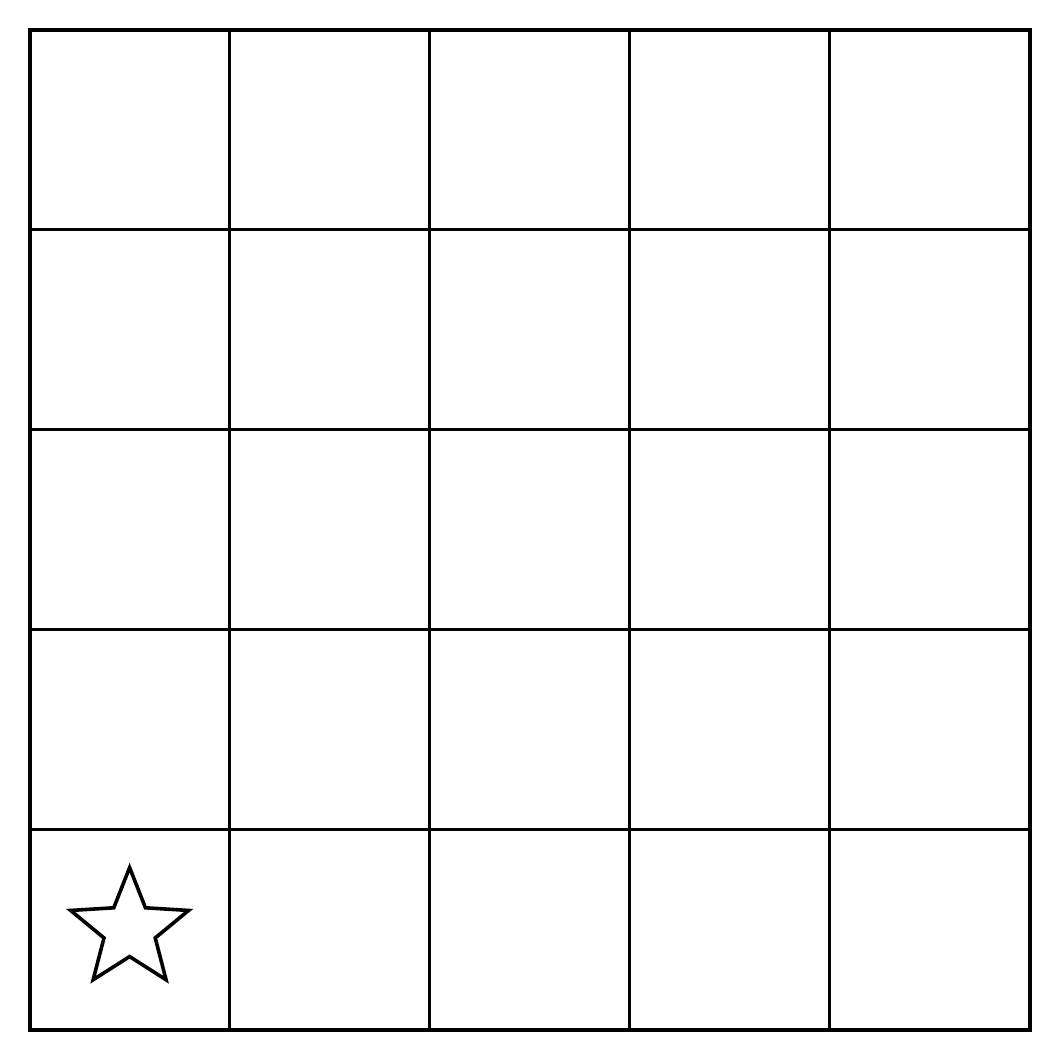
\begin{tikzpicture}[x=1in,y=1in]
\draw[line width=0.9pt] (0,0) grid[step=1] (5,5);
\draw[line width=1.4pt] (0,0) rectangle (5,5);
\node[star, star points=5, star point ratio=2.3, draw=black, line width=1.3pt, inner sep=0pt, outer sep=0pt, minimum size=0.620in] at (0.5,0.5) {};
\end{tikzpicture}}

\vspace{0.2in}
\noindent\makebox[\textwidth][c]{
\begin{tikzpicture}[x=1cm,y=1cm]
\draw[line width=1pt] (0,0) -- (10,0);
\draw[line width=1pt] (0,-0.2) -- (0,0.2);
\draw[line width=1pt] (10,-0.2) -- (10,0.2);
\node[anchor=west] at (10.3,0) {10 cm};
\end{tikzpicture}}

\newpage
\textbf{8-by-8 game board, left half, with the star.}

\vspace{0.05in}
{\small Only if your printer cuts off an edge of the 8-by-8 board on sheet 1: print one left half (sheet 3) and one right half (sheet 4) for each 8-by-8 board. Cut this half along the board's thick right edge. Lay it on the grey strip of sheet 4 so that this edge covers sheet 4's thick left edge, tape the halves together on the back, and check that the squares at the join are 1 inch.\par}

\vspace{0.14in}
\noindent\makebox[\textwidth][c]{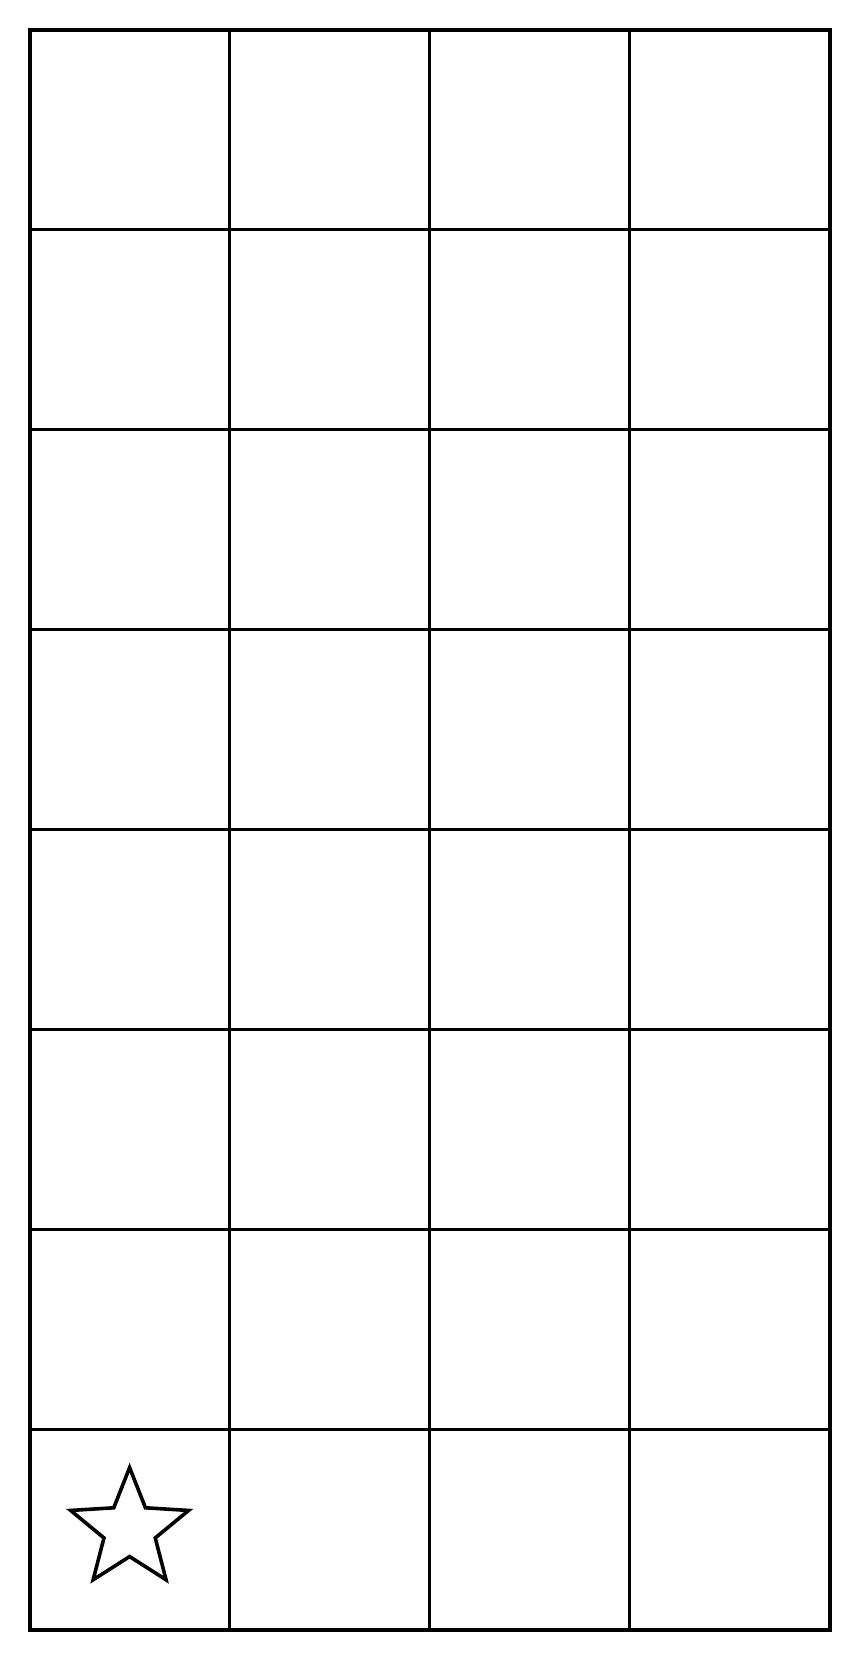
\begin{tikzpicture}[x=1in,y=1in]
\draw[line width=0.9pt] (0,0) grid[step=1] (4,8);
\draw[line width=1.4pt] (0,0) rectangle (4,8);
\node[star, star points=5, star point ratio=2.3, draw=black, line width=1.3pt, inner sep=0pt, outer sep=0pt, minimum size=0.620in] at (0.5,0.5) {};
\end{tikzpicture}}

\vspace{0.2in}
\noindent\makebox[\textwidth][c]{
\begin{tikzpicture}[x=1cm,y=1cm]
\draw[line width=1pt] (0,0) -- (10,0);
\draw[line width=1pt] (0,-0.2) -- (0,0.2);
\draw[line width=1pt] (10,-0.2) -- (10,0.2);
\node[anchor=west] at (10.3,0) {10 cm};
\end{tikzpicture}}

\newpage
\textbf{8-by-8 game board, right half.}

\vspace{0.05in}
{\small Only if your printer cuts off an edge of the 8-by-8 board on sheet 1: print one left half (sheet 3) and one right half (sheet 4) for each 8-by-8 board. The left half (sheet 3) goes on the grey strip, with its thick right edge on this board's thick left edge.\par}

\vspace{0.14in}
\noindent\makebox[\textwidth][c]{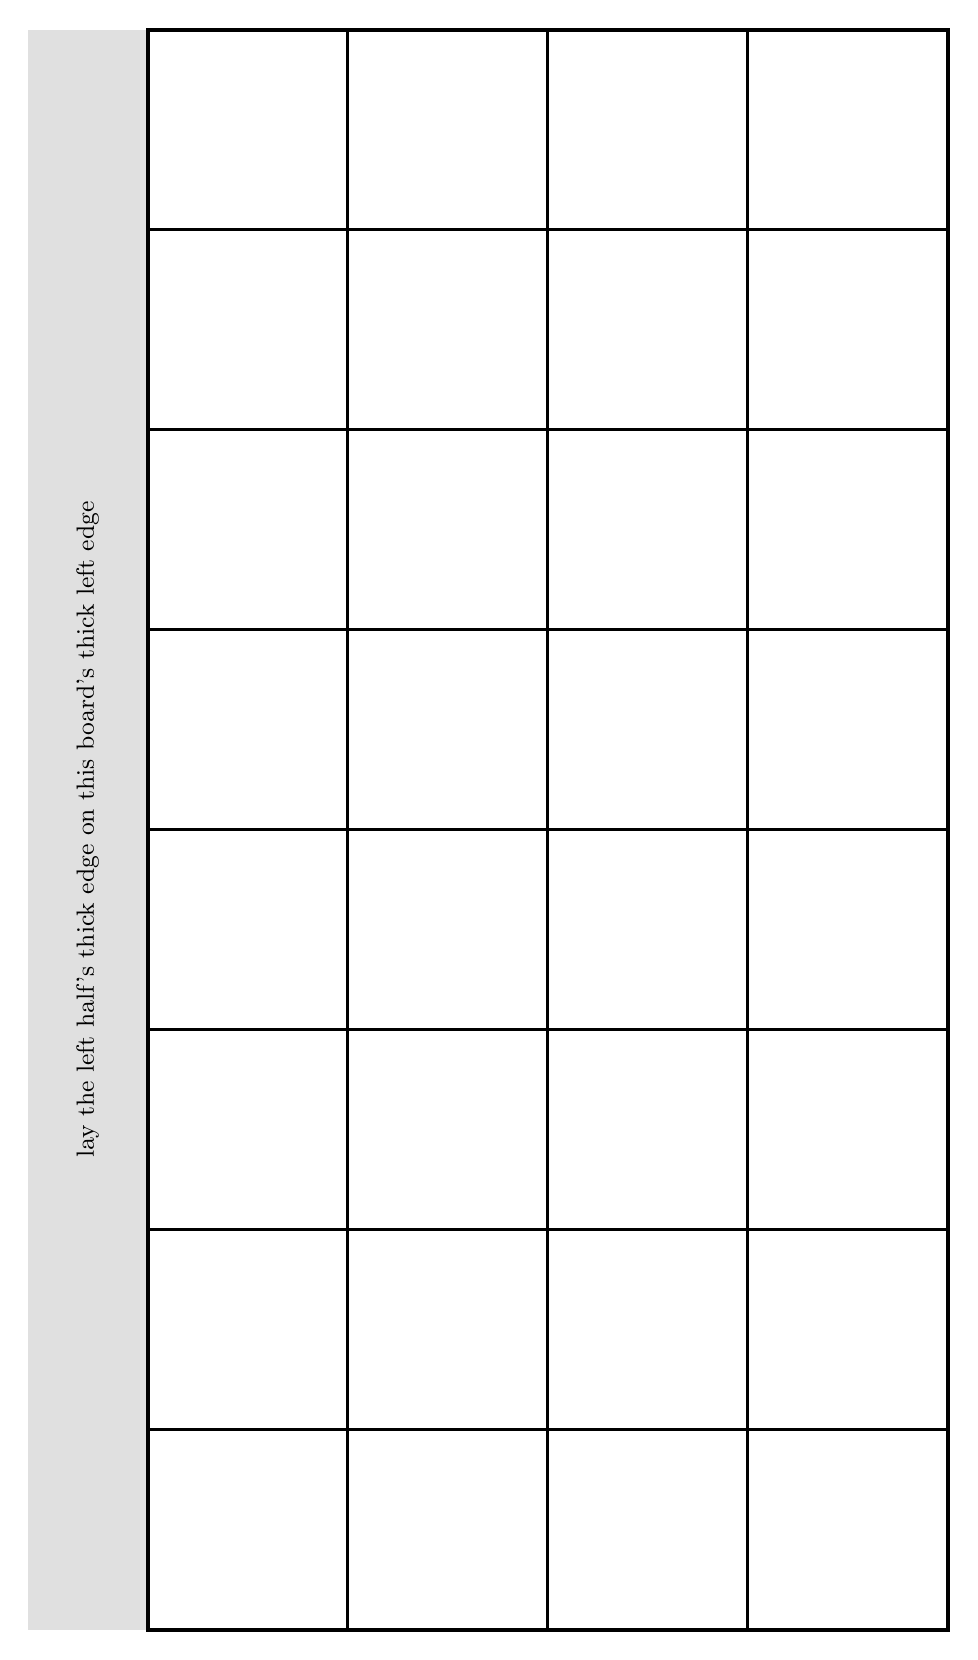
\begin{tikzpicture}[x=1in,y=1in]
\fill[black!12] (-0.6000,0) rectangle (0,8.0000);
\node[rotate=90, font=\small] at (-0.3000,4.0000) {lay the left half's thick edge on this board's thick left edge};
\draw[line width=0.9pt] (0,0) grid[step=1] (4,8);
\draw[line width=1.4pt] (0,0) rectangle (4,8);
\end{tikzpicture}}

\vspace{0.2in}
\noindent\makebox[\textwidth][c]{
\begin{tikzpicture}[x=1cm,y=1cm]
\draw[line width=1pt] (0,0) -- (10,0);
\draw[line width=1pt] (0,-0.2) -- (0,0.2);
\draw[line width=1pt] (10,-0.2) -- (10,0.2);
\node[anchor=west] at (10.3,0) {10 cm};
\end{tikzpicture}}

\newpage
\end{document}
